% =====================================================================
%  Manuscrito JSAES -- tomografia conjunta Vp + Q del Valle Medio del
%  Magdalena, con reconstruccion local de la losa de Nazca.
%
%  REGLA: ninguna cifra se escribe a mano. Todas entran por macros de
%  `cifras.tex`, que genera `genera_cifras.py` desde los JSON del
%  pipeline. Si una campana se recalcula, el texto se actualiza solo.
%
%  Ingles britanico: parameterisation, optimisation, normalisation,
%  behaviour, modelling. NO convertir a ortografia estadounidense.
% =====================================================================
\RequirePackage{cmap}
\documentclass[review,authoryear,longtitle]{elsarticle}
\usepackage[T1]{fontenc}
\usepackage{lmodern}
\usepackage{graphicx}
\usepackage{amsmath}
\usepackage{booktabs}
\usepackage{siunitx}
\usepackage{microtype}
\usepackage[a4paper,margin=25mm]{geometry}
\emergencystretch=2em
\setlength{\belowcaptionskip}{6pt}
\usepackage{placeins}
\usepackage{lineno}
\usepackage[hidelinks]{hyperref}
\pdfstringdefDisableCommands{\def\corref#1{}}
\biboptions{authoryear}
\journal{Journal of South American Earth Sciences}

\graphicspath{{figuras/}}
% Generado por paper_q1/genera_cifras.py -- NO editar a mano.
% Campaña adoptada: sgc_q_mascara_rayos_damp400

% --- red, eventos y observaciones ---
\newcommand{\estPrevia}{14}
\newcommand{\estAdoptada}{56}
\newcommand{\eventosAdoptada}{1\,114}
\newcommand{\eventosPrevia}{1\,094}
\newcommand{\picksPrevia}{4\,269}
\newcommand{\picksAdoptada}{12\,317}
\newcommand{\trazasInventario}{12\,309}
\newcommand{\trazasConEspectro}{12\,091}
\newcommand{\paresPrevia}{4\,221}
\newcommand{\paresAdoptada}{52\,957}
\newcommand{\huecoPrevio}{197.4}
\newcommand{\huecoAmpliado}{82.8}
\newcommand{\fracHuecoPrevio}{68}
\newcommand{\fracHuecoAmpliado}{5}
\newcommand{\estConLecturas}{189}
\newcommand{\fracLecturasDescartadas}{76}
\newcommand{\radioAmpliacion}{300}

% --- dominio y parametrización ---
\newcommand{\lonMinPrevia}{-74.60}
\newcommand{\lonMaxPrevia}{-72.55}
\newcommand{\latMinPrevia}{6.20}
\newcommand{\latMaxPrevia}{8.05}
\newcommand{\profMaxPrevia}{180}
\newcommand{\lonMinAdoptada}{-75.10}
\newcommand{\lonMaxAdoptada}{-72.35}
\newcommand{\latMinAdoptada}{5.30}
\newcommand{\latMaxAdoptada}{8.05}
\newcommand{\profMaxAdoptada}{140}
\newcommand{\celdasEnMascara}{2\,048}
\newcommand{\celdasIluminadas}{1\,410}
\newcommand{\celdasFueraMascaraVieja}{643}
\newcommand{\fracCeldasFuera}{46}
\newcommand{\fracImpactosFuera}{29}
\newcommand{\paresTrazados}{8\,000}

% --- regularización ---
\newcommand{\qLaplace}{3}
\newcommand{\qCellDamp}{0.05}
\newcommand{\qStationDamp}{4}
\newcommand{\qStationDampPrevio}{0.15}

% --- inversión Vp ---
\newcommand{\vpCeldasPrevia}{365}
\newcommand{\vpRmsPrevia}{0.804}
\newcommand{\vpRazonPrevia}{11.7}
\newcommand{\vpIterPrevia}{136}
\newcommand{\vpCeldasAdoptada}{907}
\newcommand{\vpRmsAdoptada}{0.635}
\newcommand{\vpRazonAdoptada}{13.6}
\newcommand{\vpIterAdoptada}{281}

% --- inversión Q ---
\newcommand{\qCeldasPrevia}{442}
\newcommand{\qRmsPrevia}{0.0617}
\newcommand{\qTerminosPrevia}{14}
\newcommand{\qRazonDatosPrevia}{9.2}
\newcommand{\qMedianaRdosPrevia}{0.128}
\newcommand{\qObsPrevia}{4\,216}
\newcommand{\qCeldasMascaraVieja}{777}
\newcommand{\qRmsMascaraVieja}{0.0607}
\newcommand{\qTerminosMascaraVieja}{56}
\newcommand{\qRazonDatosMascaraVieja}{63.5}
\newcommand{\qMedianaRdosMascaraVieja}{0.144}
\newcommand{\qObsMascaraVieja}{52\,914}
\newcommand{\qCeldasMascaraRayos}{1\,169}
\newcommand{\qRmsMascaraRayos}{0.0586}
\newcommand{\qTerminosMascaraRayos}{56}
\newcommand{\qRazonDatosMascaraRayos}{43.2}
\newcommand{\qMedianaRdosMascaraRayos}{0.144}
\newcommand{\qObsMascaraRayos}{52\,914}
\newcommand{\qCeldasAdoptada}{1\,169}
\newcommand{\qRmsAdoptada}{0.0590}
\newcommand{\qTerminosAdoptada}{56}
\newcommand{\qRazonDatosAdoptada}{43.2}
\newcommand{\qMedianaRdosAdoptada}{0.144}
\newcommand{\qObsAdoptada}{52\,914}

% --- descomposición del ajuste (la medida que vale) ---
\newcommand{\explPrevia}{12.1}
\newcommand{\razonEstPrevia}{1.08}
\newcommand{\razonEstrPrevia}{1.11}
\newcommand{\rmsDatoPrevia}{0.0702}
\newcommand{\rmsPartidaPrevia}{0.1228}
\newcommand{\rmsFinalPrevia}{0.0617}
\newcommand{\rmsRedGuionPrevia}{49.8}
\newcommand{\explMascaraVieja}{12.6}
\newcommand{\razonEstMascaraVieja}{3.74}
\newcommand{\razonEstrMascaraVieja}{3.72}
\newcommand{\rmsDatoMascaraVieja}{0.0694}
\newcommand{\rmsPartidaMascaraVieja}{0.2067}
\newcommand{\rmsFinalMascaraVieja}{0.0607}
\newcommand{\rmsRedGuionMascaraVieja}{70.6}
\newcommand{\explMascaraRayos}{15.5}
\newcommand{\razonEstMascaraRayos}{2.38}
\newcommand{\razonEstrMascaraRayos}{2.40}
\newcommand{\rmsDatoMascaraRayos}{0.0694}
\newcommand{\rmsPartidaMascaraRayos}{0.2056}
\newcommand{\rmsFinalMascaraRayos}{0.0586}
\newcommand{\rmsRedGuionMascaraRayos}{71.5}
\newcommand{\explAdoptada}{15.0}
\newcommand{\razonEstAdoptada}{1.03}
\newcommand{\razonEstrAdoptada}{1.00}
\newcommand{\rmsDatoAdoptada}{0.0694}
\newcommand{\rmsPartidaAdoptada}{0.2056}
\newcommand{\rmsFinalAdoptada}{0.0590}
\newcommand{\rmsRedGuionAdoptada}{71.3}

% --- damero ---
\newcommand{\damPerturbVp}{5}
\newcommand{\damPerturbQ}{30}
\newcommand{\damLambdas}{40, 80, 120, 160~km}
\newcommand{\damVpBajoA}{0.915}
\newcommand{\damAmpVpBajoA}{0.86}
\newcommand{\damVpObsA}{0.331}
\newcommand{\damAmpVpObsA}{1.10}
\newcommand{\damVpBajoB}{0.978}
\newcommand{\damAmpVpBajoB}{0.96}
\newcommand{\damVpObsB}{0.413}
\newcommand{\damAmpVpObsB}{1.29}
\newcommand{\damVpBajoC}{0.986}
\newcommand{\damAmpVpBajoC}{0.96}
\newcommand{\damVpObsC}{0.420}
\newcommand{\damAmpVpObsC}{1.22}
\newcommand{\damVpBajoD}{0.990}
\newcommand{\damAmpVpBajoD}{0.97}
\newcommand{\damVpObsD}{0.424}
\newcommand{\damAmpVpObsD}{1.12}
\newcommand{\damQBajoA}{0.373}
\newcommand{\damAmpQBajoA}{0.42}
\newcommand{\damTermQBajoA}{0.0062}
\newcommand{\damQObsA}{0.354}
\newcommand{\damAmpQObsA}{0.45}
\newcommand{\damTermQObsA}{0.0071}
\newcommand{\damQBajoB}{0.713}
\newcommand{\damAmpQBajoB}{0.65}
\newcommand{\damTermQBajoB}{0.0062}
\newcommand{\damQObsB}{0.672}
\newcommand{\damAmpQObsB}{0.65}
\newcommand{\damTermQObsB}{0.0071}
\newcommand{\damQBajoC}{0.820}
\newcommand{\damAmpQBajoC}{0.78}
\newcommand{\damTermQBajoC}{0.0041}
\newcommand{\damQObsC}{0.766}
\newcommand{\damAmpQObsC}{0.76}
\newcommand{\damTermQObsC}{0.0055}
\newcommand{\damQBajoD}{0.905}
\newcommand{\damAmpQBajoD}{0.86}
\newcommand{\damTermQBajoD}{0.0035}
\newcommand{\damQObsD}{0.869}
\newcommand{\damAmpQObsD}{0.84}
\newcommand{\damTermQObsD}{0.0058}
\newcommand{\damViejoQObsA}{0.328}
\newcommand{\damViejoTermQObsA}{0.0346}
\newcommand{\damViejoQObsB}{0.637}
\newcommand{\damViejoTermQObsB}{0.0221}
\newcommand{\damViejoQObsC}{0.736}
\newcommand{\damViejoTermQObsC}{0.0192}
\newcommand{\damViejoQObsD}{0.844}
\newcommand{\damViejoTermQObsD}{0.0163}

% --- techo de Q ---
\newcommand{\qTecho}{300}
\newcommand{\qTechoPrueba}{1500}
\newcommand{\fracEnTecho}{81}
\newcommand{\fracEnTechoPrueba}{64}
\newcommand{\cambioRmsTecho}{0.00000}
\newcommand{\celdasLibresTecho}{223}
\newcommand{\fracCeldasLibres}{19}
\newcommand{\qLibreMediana}{158}
\newcommand{\qLibreDiez}{64}
\newcommand{\qLibreNoventa}{260}
\newcommand{\cambioQLibre}{0.0}
\newcommand{\fracVuelveATopar}{79}
\newcommand{\qLibreZSup}{141}
\newcommand{\fracTechoZSup}{55}
\newcommand{\qLibreZVeinte}{123}
\newcommand{\fracTechoZVeinte}{76}
\newcommand{\qLibreZCuarenta}{157}
\newcommand{\fracTechoZCuarenta}{89}
\newcommand{\qLibreZCien}{176}
\newcommand{\fracTechoZCien}{97}

% --- losa de Nazca ---
\newcommand{\losaControles}{879}
\newcommand{\losaNodos}{6\,457}
\newcommand{\losaProfMin}{59}
\newcommand{\losaProfMax}{150}
\newcommand{\losaBuzamiento}{43}
\newcommand{\losaBuzamientoNoventa}{63}
\newcommand{\losaTendencia}{19}
\newcommand{\losaDistControl}{5.6}
\newcommand{\slabDifMediana}{-2.2}
\newcommand{\slabDifAbs}{8.2}
\newcommand{\slabDifNoventa}{28}
\newcommand{\slabNodos}{6\,457}

% Generated from revision_cientifica/diagnosticos.json and archived implementation.
\newcommand{\corrComponentesPrevia}{-0.919}
\newcommand{\corrComponentesMascaraVieja}{-0.989}
\newcommand{\corrComponentesMascaraRayos}{-0.976}
\newcommand{\corrComponentesAdoptada}{-0.868}
\newcommand{\nodosX}{31}
\newcommand{\pasoX}{20}
\newcommand{\nodosY}{32}
\newcommand{\pasoY}{20}
\newcommand{\nodosZ}{12}
\newcommand{\pasoZ}{20}
\newcommand{\eventosConP}{1112}
\newcommand{\fracVpTecho}{4.3}
\newcommand{\fracDeltaNegativo}{47.1}
\newcommand{\rmsQRecortado}{0.11641}
\newcommand{\rmsQRecortadoAlto}{0.10882}
\newcommand{\vpLaplace}{3}
\newcommand{\vpDamp}{0.25}
\newcommand{\lsmrMaxIter}{1200}
\newcommand{\snrMin}{3}
\newcommand{\freqMin}{1}
\newcommand{\freqMax}{12}
\newcommand{\minFrecuencias}{10}
\newcommand{\maxDelta}{0.75}
\newcommand{\pasoRayo}{2.5}
\newcommand{\inicioRuido}{-10}
\newcommand{\finRuido}{-1}
\newcommand{\inicioSenal}{0.2}
\newcommand{\finSenal}{4.2}
\newcommand{\minSenal}{2}
\newcommand{\margenS}{0.5}
\newcommand{\perfilVpInicial}{0: 5.31, 20: 7.22, 40: 8.03, 60: 8.11, 80: 8.20, 100: 8.28, 120: 8.28, 140: 8.28, 160: 8.28, 180: 8.28, 200: 8.28, 220: 8.28}
\newcommand{\perfilVpReferencia}{0: 4.74, 20: 7.25, 40: 8.81, 60: 8.51, 80: 7.83, 100: 8.28, 120: 8.28, 140: 8.28, 160: 8.28, 180: 8.28, 200: 8.28, 220: 8.28}
\newcommand{\rangoLateralVpReferencia}{1.05}
\newcommand{\nodosReferenciaX}{13}
\newcommand{\rejillaReferenciaXMin}{-186.32}
\newcommand{\rejillaReferenciaXMax}{53.68}
\newcommand{\nodosReferenciaY}{9}
\newcommand{\rejillaReferenciaYMin}{-76.21}
\newcommand{\rejillaReferenciaYMax}{83.79}
\newcommand{\nodosReferenciaZ}{12}
\newcommand{\rejillaReferenciaZMin}{0.00}
\newcommand{\rejillaReferenciaZMax}{220.00}
\newcommand{\qIterRevision}{328}
\newcommand{\semillaRayos}{20260924}
\newcommand{\lsmrTol}{10^{-6}}
\newcommand{\lsmrConlim}{10^{8}}
\newcommand{\qInicialSomero}{40}
\newcommand{\qInicialProfundo}{60}
\newcommand{\profCambioQ}{30}
\newcommand{\suavizadoLosa}{25}

% Generated from segunda_revision/diagnosticos.json
\newcommand{\auditReferenceE}{12.1128}
\newcommand{\auditReferenceStructure}{1.1093}
\newcommand{\auditReferenceStation}{1.0788}
\newcommand{\auditReferenceComponentCorr}{-0.9188}
\newcommand{\auditReferencePredictionCorr}{0.4746}
\newcommand{\auditReferenceCI}{10.22--14.15}
\newcommand{\auditReferenceInitialRms}{0.12281}
\newcommand{\auditReferenceDataRms}{0.07018}
\newcommand{\auditExpandedE}{12.5855}
\newcommand{\auditExpandedStructure}{3.8338}
\newcommand{\auditExpandedStation}{3.7366}
\newcommand{\auditExpandedComponentCorr}{-0.9895}
\newcommand{\auditExpandedPredictionCorr}{0.4875}
\newcommand{\auditExpandedCI}{10.90--14.23}
\newcommand{\auditExpandedInitialRms}{0.20672}
\newcommand{\auditExpandedDataRms}{0.06941}
\newcommand{\auditRayDomainE}{15.5116}
\newcommand{\auditRayDomainStructure}{2.3972}
\newcommand{\auditRayDomainStation}{2.3819}
\newcommand{\auditRayDomainComponentCorr}{-0.9763}
\newcommand{\auditRayDomainPredictionCorr}{0.5323}
\newcommand{\auditRayDomainCI}{14.10--16.99}
\newcommand{\auditRayDomainInitialRms}{0.20560}
\newcommand{\auditRayDomainDataRms}{0.06941}
\newcommand{\auditAdoptedE}{15.0472}
\newcommand{\auditAdoptedStructure}{0.9999}
\newcommand{\auditAdoptedStation}{1.0346}
\newcommand{\auditAdoptedComponentCorr}{-0.8680}
\newcommand{\auditAdoptedPredictionCorr}{0.5247}
\newcommand{\auditAdoptedCI}{13.65--16.51}
\newcommand{\auditAdoptedInitialRms}{0.20560}
\newcommand{\auditAdoptedDataRms}{0.06941}
\newcommand{\auditBootstrapReplicates}{10000}
\newcommand{\auditBootstrapSeed}{20261005}
\newcommand{\auditDomainGain}{2.93}
\newcommand{\auditDomainGainCI}{2.06 to 4.14}
\newcommand{\auditDampingChange}{-0.46}
\newcommand{\auditDampingChangeCI}{-0.61 to -0.33}
\newcommand{\auditInheritedVpInheritedMaskE}{12.5855}
\newcommand{\auditInheritedVpInheritedMaskRms}{0.06068}
\newcommand{\auditInheritedVpRayMaskE}{15.5060}
\newcommand{\auditInheritedVpRayMaskRms}{0.05865}
\newcommand{\auditUpdatedVpInheritedMaskE}{12.9083}
\newcommand{\auditUpdatedVpInheritedMaskRms}{0.06045}
\newcommand{\auditUpdatedVpRayMaskE}{15.5116}
\newcommand{\auditUpdatedVpRayMaskRms}{0.05865}
\newcommand{\auditMaskGainFixedVp}{2.9205}
\newcommand{\auditVelocityGainRayMask}{0.0056}
\newcommand{\auditClippedLowE}{-67.71}
\newcommand{\auditClippedHighE}{-56.77}
\newcommand{\auditLowerBoundNodes}{0}
\newcommand{\auditLowerBoundPercent}{0.0}


\begin{document}
\linenumbers
\begin{frontmatter}

\title{Auditing parameterisation and bound effects in sequential P-wave
velocity and spectral-ratio attenuation tomography of the Middle
Magdalena Valley, Colombia}

\author[inst1]{R\'omulo Sandoval Fl\'orez\corref{cor1}}
\ead{romulo@ecci.edu.co}
\author[inst2]{Francisco H. Cabrera Zambrano}
\ead{fcabrera@yahoo.com.br}
\author[inst3]{Claudia Patricia Parra Medina}
\ead{claudia.parra@unimilitar.edu.co}
\cortext[cor1]{Corresponding author.}
\address[inst1]{Universidad ECCI, Carrera 19 No. 49--20, Bogot\'a, Colombia}
\address[inst2]{Grupo de Investigaci\'on Pangea, Universidad de Pamplona, Pamplona, Colombia}
\address[inst3]{Universidad Militar Nueva Granada, Carrera 11 No. 101--80, Bogot\'a, Colombia}

\begin{abstract}
We audit parameterisation and bound effects in sequential P-wave velocity and spectral-ratio attenuation tomography of the Middle Magdalena Valley, Colombia. Servicio Geol\'ogico Colombiano data are inverted using shared straight-ray geometry, with attenuation conditioned on recovered velocity. Expanding from \estPrevia{} to \estAdoptada{} receivers increased accepted differential observations from \qObsPrevia{} to \qObsAdoptada{}, but normalised root-mean-square (RMS) reduction changed only from \explPrevia\,\% to \explMascaraVieja\,\%. Different starting fields and domains preclude isolating receiver count. An illumination audit found that \fracCeldasFuera\,\% of sampled ray-hit cells lay outside the inherited domain. Re-parameterisation increased RMS reduction to \explMascaraRayos\,\%; the paired event-bootstrap gain was \auditDomainGain{} percentage points (95\,\% interval \auditDomainGainCI), conditional on fixed predictions. A controlled mask--velocity experiment attributes almost all this gain to the mask. Stronger station damping reduced component inflation, although substantial station--structure anticorrelation persisted. Archived predictions were evaluated before model clipping. Forward RMS of the clipped attenuation model was \rmsQRecortado~s versus \rmsFinalAdoptada~s for the unconstrained solution; raising the ceiling from \qTecho{} to \qTechoPrueba{} gave \rmsQRecortadoAlto~s. Both clipped predictions fit worse than zero. Consequently, archived RMS invariance cannot establish bound non-identifiability, and below-ceiling $Q$ values remain provisional. A Benioff surface reconstructed from \losaControles{} hypocentres differed from Slab2 by a median absolute \slabDifAbs~km. These audits delimit interpretation of regional attenuation maps by requiring component-covariance diagnostics and forward evaluation of the bounded model actually displayed.
\end{abstract}

\begin{keyword}
seismic attenuation \sep local earthquake tomography \sep spectral ratio
\sep model parameterisation \sep null space \sep Nazca slab \sep Colombia
\end{keyword}

\end{frontmatter}
\clearpage

% =====================================================================
\section{Introduction}
% =====================================================================

The northern Andes record one of the most complex subduction settings in
South America, where the Nazca, Caribbean and South American plates
interact with inherited crustal structures, sedimentary basins and
strongly segmented intermediate-depth seismicity
\citep{Taboada2000,VanDerHilst1994,Syracuse2016,Schellart2023}. In
Colombia the Bucaramanga seismic nest and the surrounding
intermediate-depth seismicity constitute a dense natural source array, yet
the relation between hypocentral patterns, elastic anomalies and plate
geometry remains scale dependent
\citep{Zarifi2007,Londono2019,SepulvedaJaimes2018,Hayes2018Slab2}.
Attenuation is in principle a sharper discriminant than velocity for
temperature, partial melt and fluid content
\citep{Hacker2003,Mavko2009,vanKeken2011}, which motivates
$Q$ imaging as a complement to velocity tomography in this setting.

The MMV is an intermontane basin between the Central and Eastern
Cordilleras, bounded and crossed by inherited fault systems and filled by
Cenozoic clastic sequences that strongly depress shallow seismic
velocities and distort local ray geometry
\citep{MojicaFranco1990,GomezTapias2019}. The structural framework
includes the Bucaramanga--Santa Marta, La Salina and Eastern Frontal fault
systems, which link basin inversion, Andean shortening and dextral
deformation of the North Andean block
\citep{MojicaFranco1990,Audemard2021,Muller2010}. Earlier work
established the regional catalogue, the local magnitude scale and
crustal-to-upper-mantle velocity structure from ambient-noise and
arrival-time inversion
\citep{OjedaHavskov2001,Poveda2018,LondonoRomero2017,Londono2020Velocity,HavskovOttemoller2010},
and more recently regional attenuation estimates
\citep{Londono2022Attenuation,CastelblancoOssa2023,Castelblanco2025Attenuation}.
The configuration is unfavourable in a specific way: basin heterogeneity,
receiver-side site response and intermediate-depth sources are sampled by
one elongated network, so receiver terms and path structure compete for
the same observations.

Local earthquake tomography relates arrival-time residuals to
three-dimensional structure through a linearised inverse problem
\citep{Aki1976,Crosson1976,Thurber1983,Pavlis1980}, and the
spectral-ratio method extends this to attenuation by cancelling the common
source spectrum between two receivers of a single event
\citep{AndersonHough1984,QuanHarris1997,Safak1997,EberhartPhillipsChadwick2002}.
In both cases the recovered structure is conditioned by the
parameterisation: unsampled cells are undetermined, and parameters that
trade off against one another are individually meaningless even where
their combination fits the data
\citep{Thurber1992,Zhao2015,Menke2018,Rawlinson2016}. For spectral-ratio
$Q$ the trade-off is acute. Station terms enter every observation with
opposite sign, so their mean is unconstrained and their differences can
absorb any path effect the parameterised volume cannot express
\citep{EberhartPhillipsChadwick2002,GuoThurber2021,GaoWang2016}.

The station--structure trade-off and inverse non-uniqueness are established
in the literature cited above. Our contribution is to make their audit
explicit and reproducible in a sequential, bounded-model workflow: report
component covariance on the retained observations; distinguish invariance
of an archived residual from non-identifiability of a bound; and evaluate
the forward prediction of the actual bounded model before interpreting it.
The reference and expanded campaigns illustrate why receiver count alone
is insufficient, although their different starting fields and grids
prevent a receiver-only comparison. Paired event resampling quantifies
sampling variability of the archived fit, and a controlled mask--velocity
experiment isolates the parameterisation effect. A damping sweep and
structure-only synthetic tests diagnose remaining coupling. The Middle
Magdalena models and a seismicity-defined Benioff surface compared with
Slab2 \citep{Hayes2018Slab2} serve as a case study; the clipped attenuation
values remain provisional.

% =====================================================================
\section{Tectonic setting and data}
% =====================================================================

\subsection{Seismological data}

All data derive from the Servicio Geol\'ogico Colombiano national network.
The inventory contains \eventosAdoptada{} events with QuakeML phase
information and archived waveforms; \eventosConP{} have retained
P-wave picks and appear in the location map. They yield \picksAdoptada{} P-wave
arrival times for the velocity branch. For the attenuation branch,
\trazasInventario{} vertical-component records were retrieved, of which
\trazasConEspectro{} yielded usable signal and noise spectra after
instrument-response deconvolution using SGC StationXML poles and zeros.
Pairing within events produced \paresAdoptada{} differential $t^{*}$
observations, of which \qObsAdoptada{} passed quality control and enter
the inversion. The reference campaign similarly produced \paresPrevia{}
pairs, of which \qObsPrevia{} were accepted. Raw and accepted counts
are kept distinct throughout.

\subsection{Receiver configuration}

An inventory of the archived QuakeML shows P-phase picks at
\estConLecturas{} stations for these events, whereas the reference
configuration defined here used \estPrevia;
the domain filter discarded \fracLecturasDescartadas\,\% of available
picks. Retaining all stations within \radioAmpliacion{}~km yields
\estAdoptada{} receivers, reduces the median azimuthal gap per event from
\huecoPrevio$^{\circ}$ to \huecoAmpliado$^{\circ}$, and reduces the
proportion of events with gap $>180^{\circ}$ from \fracHuecoPrevio\,\% to
\fracHuecoAmpliado\,\%. Section~\ref{sec:cobertura} shows that
the reference-to-expanded campaign comparison produces little improvement
in the archived linear fit.

\begin{figure}[t]
  \centering
  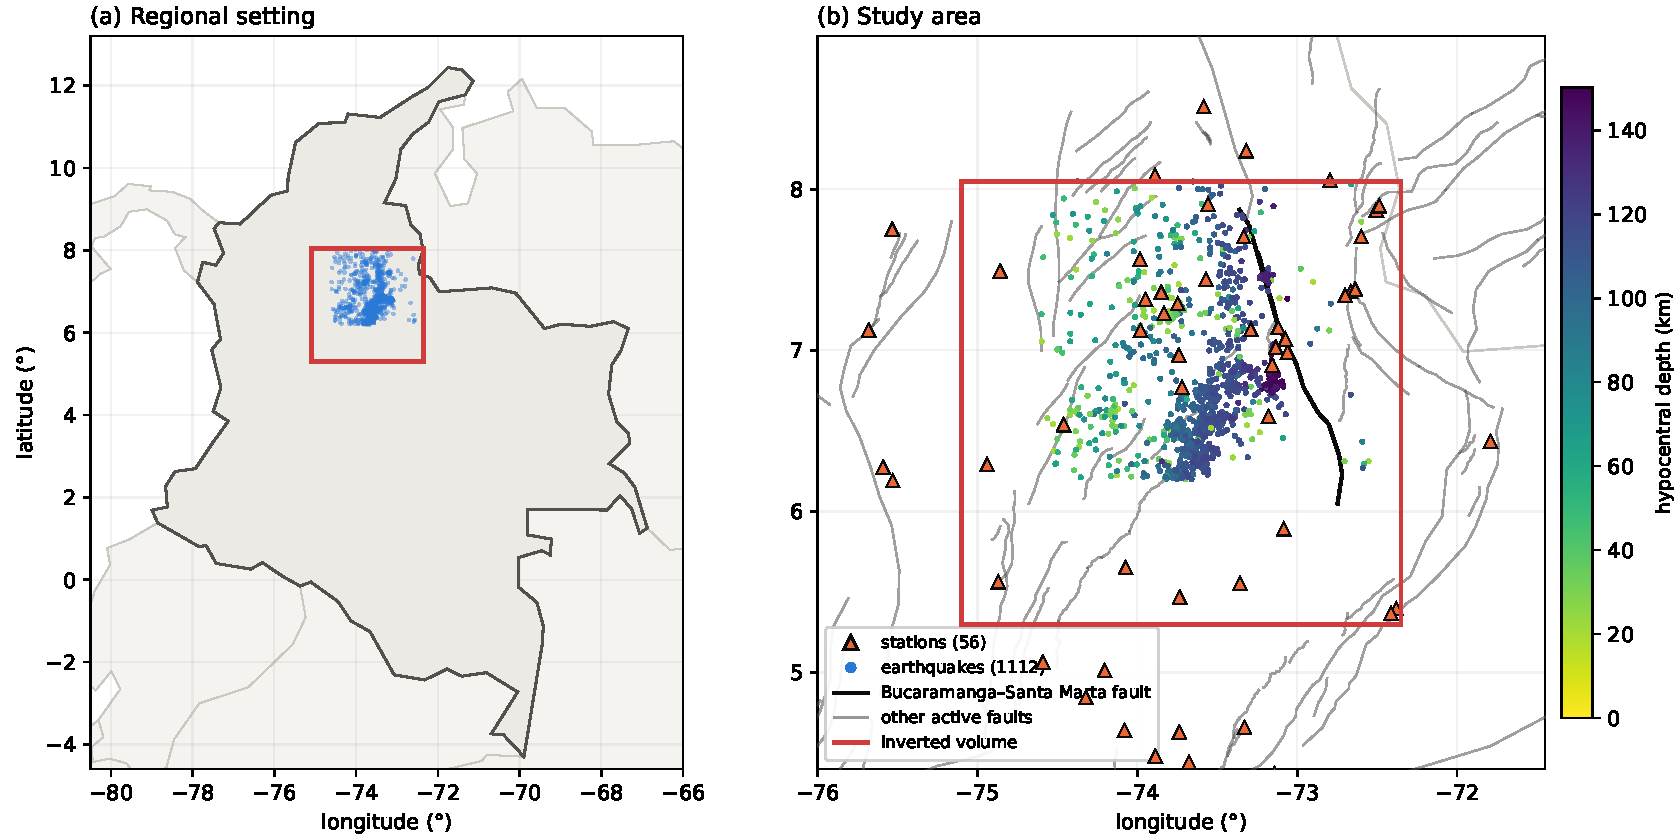
\includegraphics[width=1.0\linewidth]{mapa_situacion.pdf}
  \caption{Location of the study area. (a) Regional setting, with the inverted volume outlined in red and the full earthquake set in blue. (b) Enlargement of that volume showing the \eventosConP{} earthquakes with retained P-wave picks, coloured by hypocentral depth, the \estAdoptada{} receivers (triangles), and active fault traces from the GEM database \citep{StyronPagani2020}; the Bucaramanga--Santa Marta system is highlighted. The elongation of the permanent network along the basin axis is the geometric origin of the station--structure trade-off analysed in Section~\ref{sec:descomposicion}.}
  \label{fig:mapa}
\end{figure}

% =====================================================================
\section{Method}
% =====================================================================

\subsection{Grids and starting models}

Both branches in the expanded campaigns use a regular Cartesian grid with spacing
\SI{\pasoX}{\kilo\metre}, containing \nodosX{} by \nodosY{} by
\nodosZ{} nodes along $x$, $y$ and depth, respectively. Only nodes inside
the campaign domain and above the hit threshold are inverted; the full
computational grid must therefore be distinguished from the active mask.
The reference domain extends from $\lonMinPrevia^{\circ}$ to
$\lonMaxPrevia^{\circ}$ longitude, $\latMinPrevia^{\circ}$ to
$\latMaxPrevia^{\circ}$ latitude and to \profMaxPrevia~km depth.
It uses \estPrevia{} receivers, \picksPrevia{} P picks and
\qObsPrevia{} accepted spectral pairs on a computational grid of
\nodosReferenciaX{} by \nodosReferenciaY{} by \nodosReferenciaZ{} nodes,
also at nominal \SI{\pasoX}{\kilo\metre} spacing. Its computational
$x$ range is \rejillaReferenciaXMin{} to \rejillaReferenciaXMax~km,
and $y$ range \rejillaReferenciaYMin{} to \rejillaReferenciaYMax~km,
relative to the common geographic origin. Computational extent and the
nominal rectangular inversion domain are distinct ray constraints.
Its archived starting velocity field is three-dimensional, with maximum
within-layer range \rangoLateralVpReferencia~km~s$^{-1}$; the expanded
campaigns instead use the one-dimensional profile below. The reference
comparison therefore changes receivers, computational support and starting
velocity structure together, and is not a controlled receiver-only test.
The complete reference starting field is retained in the model archive.
The ray-consistent domain is
specified in Section~\ref{sec:parametrizacion}. The same straight-ray
operator, hit thresholds and regularisation weights are used for the
reference and expanded comparisons, apart from the declared station
damping sweep. In the ray-consistent comparison, changing the domain
also changes the recovered velocity field used in the attenuation
kernel; this is a sequential effect, not an isolated change of the
attenuation mask.

All grids have vertical nodes at 0, 20, 40, 60, 80, 100, 120, 140,
160, 180, 200 and 220~km. Computational storage therefore extends beyond
the declared inversion domains. Nodes deeper than the respective domain
limits are inactive and retain their starting values. The deepest active
velocity and attenuation nodes in both inherited-domain campaigns are at
160~km, because activation additionally requires the hit threshold; in the
ray-domain campaigns both branches extend to 140~km. A 220~km storage
extent does not imply resolution to that depth.

The expanded campaigns' starting velocity profile is given as depth in km:
velocity in km~s$^{-1}$, \perfilVpInicial. Initial $Q$ is
\qInicialSomero{} above \profCambioQ~km and \qInicialProfundo{} below.
Velocity nodes with at least ten ray hits and attenuation nodes with at
least five are active. Velocity smoothing and damping weights are
$\lambda_L=\vpLaplace$ and $\lambda_D=\vpDamp$; attenuation cell smoothing
and damping are \qLaplace{} and \qCellDamp. The original station damping
is \qStationDampPrevio{} and the adopted value is \qStationDamp.
These are multipliers of the augmented least-squares rows; their numerical
values are tied to the operator units and are not directly transferable
to another discretisation.

LSMR uses the implementation's default tolerances
$\mathrm{atol}=\mathrm{btol}=\lsmrTol$ and condition limit
$\mathrm{conlim}=\lsmrConlim$, with at most \lsmrMaxIter{} iterations.
The adopted velocity and attenuation runs terminate after
\vpIterAdoptada{} and \qIterRevision{} iterations with stopping code two
(least-squares tolerance met). Rays are straight segments sampled every
\pasoRayo~km; velocity is solved first and then held fixed in the
attenuation kernel. There is no common objective or iterative feedback
from attenuation to velocity.

\subsection{Velocity branch}

Travel-time perturbations are related to slowness perturbations by
$\delta t = \sum_k \ell_k\,\delta s_k$, with $\ell_k$ the path length in
cell $k$ \citep{Aki1976,Thurber1983,Cerveny2001}. The system is solved
with LSMR \citep{FongSaunders2011} under Laplacian smoothing and damping,
%
\begin{equation}
  \min_{\delta \mathbf{s}}
  \left\|
  \begin{bmatrix} \mathbf{A} \\ \lambda_{L}\mathbf{L} \\
                  \lambda_{D}\mathbf{I} \end{bmatrix} \delta \mathbf{s}
  -
  \begin{bmatrix} \mathbf{d} \\ \mathbf{0} \\ \mathbf{0} \end{bmatrix}
  \right\|_{2}^{2} .
  \label{eq:vp}
\end{equation}
%
Velocity regularisation weights are fixed across campaigns. The
attenuation station damping varies only in the declared sweep.
After solving, velocities are clipped to the numerical interval
2--15~km~s$^{-1}$; \fracVpTecho\,\% of active velocity nodes reach the
upper limit. This generous upper limit is a numerical safeguard, not a
plausible lithospheric velocity or a validated physical constraint.
The archived residuals refer to the solution before this clipping.

\subsection{Spectral-ratio attenuation branch}

For one event recorded at stations $i$ and $j$, the amplitude-spectral
ratio cancels the source term, giving
%
\begin{equation}
  \ln \frac{A_i(f)}{A_j(f)} = c - \pi f \, \Delta t^{*}_{ij},
  \qquad
  \Delta t^{*}_{ij} = \int_{\mathrm{ray}\,i}\!\frac{\mathrm{d}\ell}{V\!Q}
                    - \int_{\mathrm{ray}\,j}\!\frac{\mathrm{d}\ell}{V\!Q},
  \label{eq:tstar}
\end{equation}
%
so that $\Delta t^{*}_{ij}$ equals minus the fitted slope divided by $\pi$ \citep{AndersonHough1984,QuanHarris1997}. Spectra are computed
over a signal window from \inicioSenal{} to \finSenal~s after
the P onset, truncated \margenS~s before the estimated S arrival
and requiring at least \minSenal~s of usable signal. The equally
processed noise window spans \inicioRuido{} to \finRuido~s relative
to the P onset;
the fit is restricted to frequencies at which both records exceed a
signal-to-noise threshold. The candidate band is \freqMin--\freqMax~Hz,
restricted below the sampling-dependent Nyquist limit; at least
\minFrecuencias{} bins must meet amplitude SNR $\ge\snrMin$ at both
receivers. All distinct pairs of available spectra within each event are
fitted by ordinary least squares. Non-finite estimates and
$|\Delta t^*|>\maxDelta$~s are rejected; there is no additional $R^2$
cutoff or uncertainty weighting. The retained signed differences include
\fracDeltaNegativo\,\% negative values, which are permissible because
station ordering, not path length, defines their sign. A low spectral
$R^2$ remains a limitation: many pairs share a record and cannot be treated
as independent evidence. The inversion solves jointly for cell
perturbations and one term per station,
%
\begin{equation}
  \Delta t^{*}_{ij}-\Delta t^{*}_{0,ij}
  = \sum_k G_{ij,k}\,\delta q_k + \tau_i - \tau_j ,
  \qquad G_{ij,k}=\frac{\ell^{\,i}_k-\ell^{\,j}_k}{V_k},
  \label{eq:qinv}
\end{equation}
%
where $\delta q_k$ is the perturbation in $Q_k^{-1}$, $V_k$ is the
fixed recovered velocity, and $\Delta t^*_{0,ij}$ is the starting-model
prediction including paths outside the active mask. The station term
$\tau$ absorbs receiver, coupling, site and residual-instrument
contributions \citep{EberhartPhillipsChadwick2002}. Since $\tau_i$ and
$\tau_j$ enter with opposite sign, only their differences are determined.

\begin{figure}[t]
  \centering
  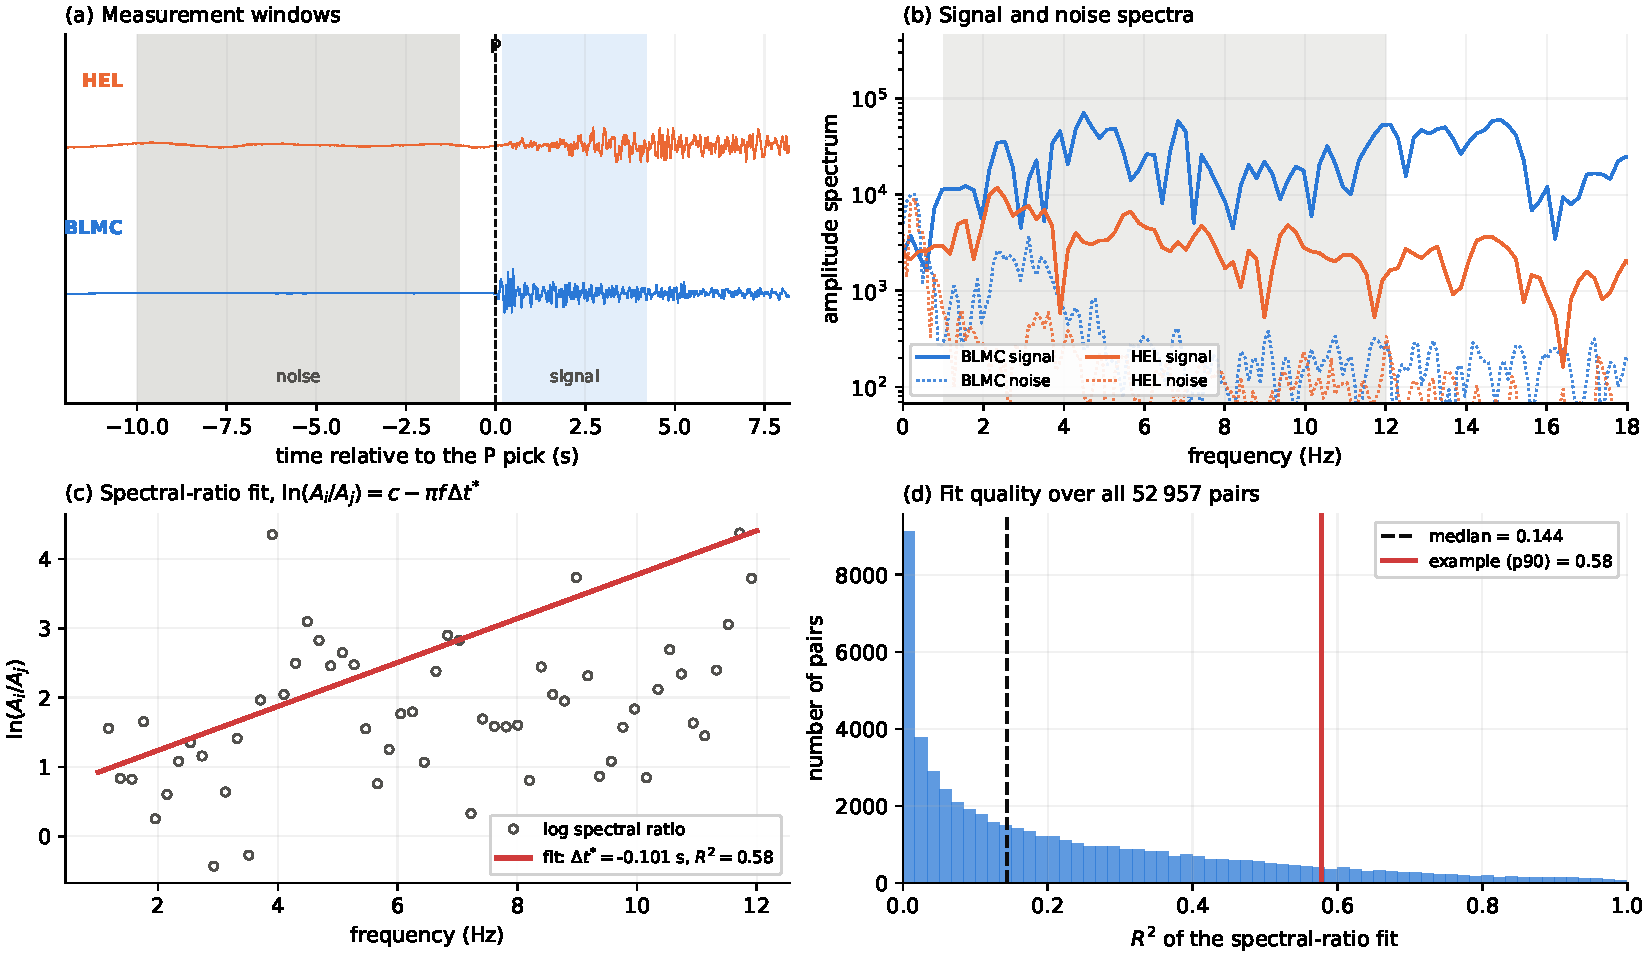
\includegraphics[width=1.0\linewidth]{metodo_espectral.pdf}
  \caption{Measurement of a differential $t^{*}$. (a) Vertical-component records at two stations of one event, with the noise and signal windows used for the spectra; traces are normalised and offset. (b) Amplitude spectra of signal (solid) and noise (dotted) for both stations; the shaded band is the frequency range over which the ratio is fitted. (c) Logarithmic spectral ratio and its linear fit, whose slope gives $\Delta t^{*}$ through Equation~\ref{eq:tstar}. (d) Distribution of the fit $R^{2}$ over all pairs, with the median and the example of panels (a)--(c) marked. The example was selected by declared percentile of $R^{2}$, not by inspection; the median of \qMedianaRdosAdoptada{} indicates that most individual measurements are weak, which limits individual estimates. The number of pairs does not remove their shared-record dependence or establish unbiased attenuation.}
  \label{fig:metodo}
\end{figure}

\subsection{Decomposition diagnostic}
\label{sec:descomposicion}

The archived statistic is normalised RMS reduction relative to a zero
prediction, not normalised RMS reduction:
\begin{equation}
 E_{\rm RMS}=100\left(1-
 \frac{\sqrt{N^{-1}\sum_n(d_n-\hat d_n)^2}}
      {\sqrt{N^{-1}\sum_n d_n^2}}\right).
 \label{eq:nrms}
\end{equation}
It differs from $R^2$ and from the prediction-to-data variance ratio.
Normalising by the data avoids dependence on a poor starting model, but
does not measure how uniquely its components are determined. We partition
the complete unconstrained linear prediction, including the starting
contribution, as
\begin{equation}
 \hat d_n=\underbrace{d_{0,n}+\sum_k G_{n,k}\delta q_k}_{c_n}
       +\underbrace{\tau_i-\tau_j}_{u_n}.
 \label{eq:descomp}
\end{equation}
All component standard deviations and covariances use the same retained
observations. They obey the exact centred identity
\begin{equation}
 \operatorname{Var}(\hat d)=\operatorname{Var}(c)+
 \operatorname{Var}(u)+2\operatorname{Cov}(c,u).
 \label{eq:covariance}
\end{equation}
The two standard-deviation ratios indicate component inflation; values
near unity alone do not establish good conditioning or independence.
We therefore also report their correlation. Strong anticorrelation with
large component amplitudes is evidence of cancellation, consistent with
a station--structure trade-off \citep{Menke2018}. It is a diagnostic,
not a direct estimate of the operator's condition number.
These diagnostics describe the unconstrained least-squares prediction,
not forward predictions from the subsequently clipped model.
The fit statistic and all moments in Table~\ref{tab:campanas} use exactly
the same retained observation vector for each campaign. Since the
solution minimises an augmented, regularised objective, the data residual
is not necessarily orthogonal to the prediction. The centred variance
identity therefore does not imply an ordinary-least-squares relation
between $E_{\rm RMS}$ and prediction variance. We also report
$\operatorname{Corr}(\hat d,d)$.

To estimate sampling variability we draw \auditBootstrapReplicates{}
bootstrap samples of events with replacement, retaining all pairs from
each sampled event together (seed \auditBootstrapSeed). We report the
2.5th and 97.5th percentiles of $E_{\rm RMS}$. Expanded-domain comparisons
share exactly the same pairs, so their contrasts use the same event draw
in both configurations. The reference population is resampled separately.
These intervals condition on the archived predictions: the models are not
refitted. They account for within-event dependence, but not shared-station
dependence across events, parameter uncertainty or systematic errors, and
are not confidence intervals for individual tomographic values.

\subsection{Ray-consistent parameterisation}

Illumination is measured by tracing the rays of \paresTrazados{}
accepted spectral-ratio pairs through the grid and counting cell hits.
The pairs are selected by random sampling without replacement with seed
\semillaRayos. Rays are straight, and their geometric paths do not bend
in either the initial or final velocity model; the latter enters only
as a travel-time/attenuation weight. The inverted
volume is then defined to contain the illumination rather than inherited
from the nominal study area. The mask is changed in
the original campaign comparison, and the sequential velocity recomputation
also changes attenuation weights. The illumination audit counts nodes
with at least one hit among the sampled pairs. This is the rounded,
sample-scaled threshold $\max[1,\operatorname{round}(5\times
\paresTrazados/\qObsAdoptada)]=1$, distinct from the five-hit activation
criterion applied to the complete inversion dataset. A sampled hit is
evidence of geometric coverage, not sufficient evidence of resolution.

We additionally perform a controlled two-by-two attenuation experiment:
each inherited or ray-domain active mask is combined with each saved
inherited or updated velocity field. The grid, retained pairs, starting
$Q$, quadrature and original regularisation, including station damping
\qStationDampPrevio, remain fixed. Only the selected mask and velocity
weights change. These are new unconstrained linear fits, not bounded
inversions; their two diagonal cases reproduce archived residual RMS to
within $10^{-7}$~s (maximum pointwise prediction difference below
$10^{-4}$~s). Small floating-point summation differences change the LSMR
stopping iteration without materially changing the fit.

\subsection{Regularisation}

Station damping $\lambda_\tau$ is swept over more than two orders of
magnitude. The adopted value balances reduced component inflation against
loss of normalised RMS reduction \citep{Hansen1992,Menke2018}. This is
an empirical choice within the tested sweep, not proof of an optimum or
complete elimination of non-uniqueness. Structure-only synthetic tests
provide a separate check on leakage into station terms.

\subsection{Resolution tests}

Checkerboard patterns are imposed with sign
$(-1)^{\lfloor i/n\rfloor + \lfloor j/n\rfloor + \lfloor k/n\rfloor}$ on
grid indices, giving a declared wavelength of $2n$ grid spacings, and are
repeated at \damLambdas{} because a single scale cannot distinguish a
resolved model from a smoothed one \citep{Leveque1993,Rawlinson2016}.
Synthetic data are generated on the final geometry and inverted under the
regularisation of the reported model. Two noise levels are used: a low
level and a level equal to the adopted campaign's archived residual RMS
before clipping (attenuation \rmsFinalAdoptada~s; velocity
\vpRmsAdoptada~s). These are declared
noise scenarios, not rigorous bounds on true resolution, because the
residual contains unmodelled signal and the simulated noise does not
represent shared-record errors. For the attenuation branch the synthetic data
contain structure only, with $\tau\equiv0$, so that the test additionally
measures how much structure the free station terms absorb.

\subsection{Model clipping and ceiling sensitivity}

The archived implementation solves an unconstrained linear least-squares
system and then clips $Q^{-1}$ to the interval corresponding to
$20\le Q\le\qTecho$. It does not solve a bound-constrained objective.
Its stored prediction is evaluated from the unconstrained perturbation,
before clipping. Changing the ceiling to \qTechoPrueba{} therefore cannot
alter that stored RMS when the linear system is unchanged.
We evaluate both saved clipped models with the same straight-ray operator
and station terms, and report this forward RMS separately. Ceiling
saturation is retained as a flag for sensitivity to the numerical bound,
but equal archived RMS values cannot demonstrate that the data fail to
constrain the upper range of $Q$.

\subsection{Benioff-surface reconstruction}

Intermediate-depth hypocentres lying within active velocity cells serve as
controls for a thin-plate-spline surface with smoothing parameter
\suavizadoLosa{} in the kilometre coordinate system, evaluated inside the convex hull
of the controls. Geometry is defined by seismicity alone; velocity and
attenuation are sampled on the resulting surface by trilinear
interpolation; active-mask membership uses the nearest grid node.
The fine surface sampling describes hypocentral geometry, not finer
tomographic resolution. Interpolation across a \SI{\pasoX}{\kilo\metre}
grid can mix active and inactive or clipped nodes, so attribute maps
are descriptive rather than independent measurements at each surface node. Using $Q$
to constrain the surface on which $Q$ is subsequently read would be
circular and is avoided. Local dip is obtained from the surface gradient;
a single plane fitted to the whole surface averages steep and gentle
segments and is reported only as an overall trend. The surface is compared
with Slab2 \citep{Hayes2018Slab2}, as an external benchmark. Overlap between source catalogues has not been
excluded, so statistical independence of the two surfaces is not assumed.

% =====================================================================
\section{Results}
% =====================================================================

\subsection{Reference and expanded campaign comparison}
\label{sec:cobertura}

Expanding the network increased the spectral-ratio dataset by more than an
order of magnitude and the number of active attenuation cells from
\qCeldasPrevia{} to \qCeldasMascaraVieja, yet normalised RMS reduction moved
only from \explPrevia\,\% to \explMascaraVieja\,\%
(Table~\ref{tab:campanas}). Conventional RMS reduction is
\rmsRedGuionPrevia\,\% relative to a starting residual RMS of
\auditReferenceInitialRms~s in the reference campaign, and
\rmsRedGuionMascaraVieja\,\% relative to
\auditExpandedInitialRms~s in the expanded campaign. Their respective
data RMS values are \auditReferenceDataRms{} and
\auditExpandedDataRms~s. These reductions use different starting
predictions, generated by the respective three-dimensional and
one-dimensional starting velocity fields. They measure improvement over
different baselines and cannot by themselves compare goodness of fit
across the campaigns.

The decomposition of Equation~\ref{eq:descomp} resolves the discrepancy.
In the reference configuration the structural and station contributions
had ratios \razonEstrPrevia{} and \razonEstPrevia{} relative to the data.
After expansion these rose to \razonEstrMascaraVieja{} and
\razonEstMascaraVieja. Their correlation changes from
\corrComponentesPrevia{} in the reference campaign to
\corrComponentesMascaraVieja{} after expansion, confirming increased
cancellation in the complete linear prediction.

\begin{table}[t]
  \centering
  \caption{Attenuation diagnostics on the same retained observations within
  each row. Panel (a) reports normalised RMS reduction and conditional
  event-bootstrap 95\,\% intervals; panel (b) gives component moments and
  correlations for the complete unconstrained prediction. Expanded rows
  share the same observation vector; the reference uses a different one.
  Cells denote active attenuation nodes.}
  \label{tab:campanas}
  \begin{tabular}{lrrrrl}
    \toprule
    (a) Configuration & Stations & Obs. & Cells & $E_{\rm RMS}$ (\%) & 95\,\% interval \\
    \midrule
    Reference & \estPrevia & \qObsPrevia & \qCeldasPrevia
      & \auditReferenceE & \auditReferenceCI \\
    Expanded, inherited domain & \estAdoptada & \qObsAdoptada
      & \qCeldasMascaraVieja & \auditExpandedE & \auditExpandedCI \\
    Ray-consistent domain & \estAdoptada & \qObsAdoptada
      & \qCeldasAdoptada & \auditRayDomainE & \auditRayDomainCI \\
    Adopted ($\lambda_{\tau}=\qStationDamp$) & \estAdoptada
      & \qObsAdoptada & \qCeldasAdoptada & \auditAdoptedE & \auditAdoptedCI \\
    \bottomrule
  \end{tabular}
  \par\medskip
  \begin{tabular}{lrrrr}
    \toprule
    (b) Configuration & $\sigma_c/\sigma_d$ & $\sigma_u/\sigma_d$
      & $\operatorname{Corr}(c,u)$ & $\operatorname{Corr}(\hat d,d)$ \\
    \midrule
    Reference & \auditReferenceStructure & \auditReferenceStation & \auditReferenceComponentCorr & \auditReferencePredictionCorr \\
    Expanded, inherited domain & \auditExpandedStructure & \auditExpandedStation & \auditExpandedComponentCorr & \auditExpandedPredictionCorr \\
    Ray-consistent domain & \auditRayDomainStructure & \auditRayDomainStation & \auditRayDomainComponentCorr & \auditRayDomainPredictionCorr \\
    Adopted ($\lambda_\tau=\qStationDamp$) & \auditAdoptedStructure & \auditAdoptedStation & \auditAdoptedComponentCorr & \auditAdoptedPredictionCorr \\
    \bottomrule
  \end{tabular}
\end{table}

\subsection{Illumination and parameterisation}
\label{sec:parametrizacion}

Tracing \paresTrazados{} pairs shows that \celdasIluminadas{} cells
receive rays, of which \celdasFueraMascaraVieja{}
(\fracCeldasFuera\,\%) lie outside the inherited domain and carry
\fracImpactosFuera\,\% of all hits. Frozen at the one-dimensional starting
model, their misfit can be accommodated only by the station terms, which
is the behaviour the decomposition detects.

Re-parameterising over the illuminated volume
(longitude $\lonMinAdoptada^{\circ}$ to $\lonMaxAdoptada^{\circ}$, latitude
$\latMinAdoptada^{\circ}$ to $\latMaxAdoptada^{\circ}$, depth to \profMaxAdoptada~km;
\celdasEnMascara{} cells), retaining the spectral pairs and regularisation
but recomputing velocity before attenuation,
raised normalised RMS reduction to \explMascaraRayos\,\%, reduced the trade-off
ratios to \razonEstrMascaraRayos{} and \razonEstMascaraRayos, and
increased active attenuation nodes to \qCeldasAdoptada. The velocity
branch has \vpCeldasAdoptada{} active nodes and archived linear RMS
\vpRmsAdoptada~s. The reference has \vpCeldasPrevia{} active nodes,
but its different data and starting field preclude interpreting the count
increase alone as improved velocity accuracy.

The paired event-bootstrap increase from the inherited to the ray-domain
campaign is \auditDomainGain{} percentage points, with conditional
95\,\% interval \auditDomainGainCI. The interval excludes zero under
this resampling scheme, while its scope is limited to the fixed-prediction
comparison described above. The controlled experiment
(Table~\ref{tab:controlled}) separates the mask and sequential velocity
effects. At fixed inherited velocity, switching to the ray mask increases
$E_{\rm RMS}$ by \auditMaskGainFixedVp{} percentage points. Updating the
velocity within that mask adds only \auditVelocityGainRayMask{} points.
The masking effect dominates this comparison, although the two factors
interact and this result does not validate a bounded attenuation map.

\begin{table}[t]
\centering
\caption{Controlled attenuation fits on the same retained pairs, with
original station damping. Only the active mask and saved velocity weights
vary; fit statistics refer to unconstrained linear predictions.}
\label{tab:controlled}
\begin{tabular}{llrr}
\toprule
Velocity weights & Active mask & $E_{\rm RMS}$ (\%) & Residual RMS (s) \\
\midrule
Inherited & Inherited & \auditInheritedVpInheritedMaskE & \auditInheritedVpInheritedMaskRms \\
Inherited & Ray domain & \auditInheritedVpRayMaskE & \auditInheritedVpRayMaskRms \\
Updated & Inherited & \auditUpdatedVpInheritedMaskE & \auditUpdatedVpInheritedMaskRms \\
Updated & Ray domain & \auditUpdatedVpRayMaskE & \auditUpdatedVpRayMaskRms \\
\bottomrule
\end{tabular}
\end{table}

\begin{figure}[t]
  \centering
  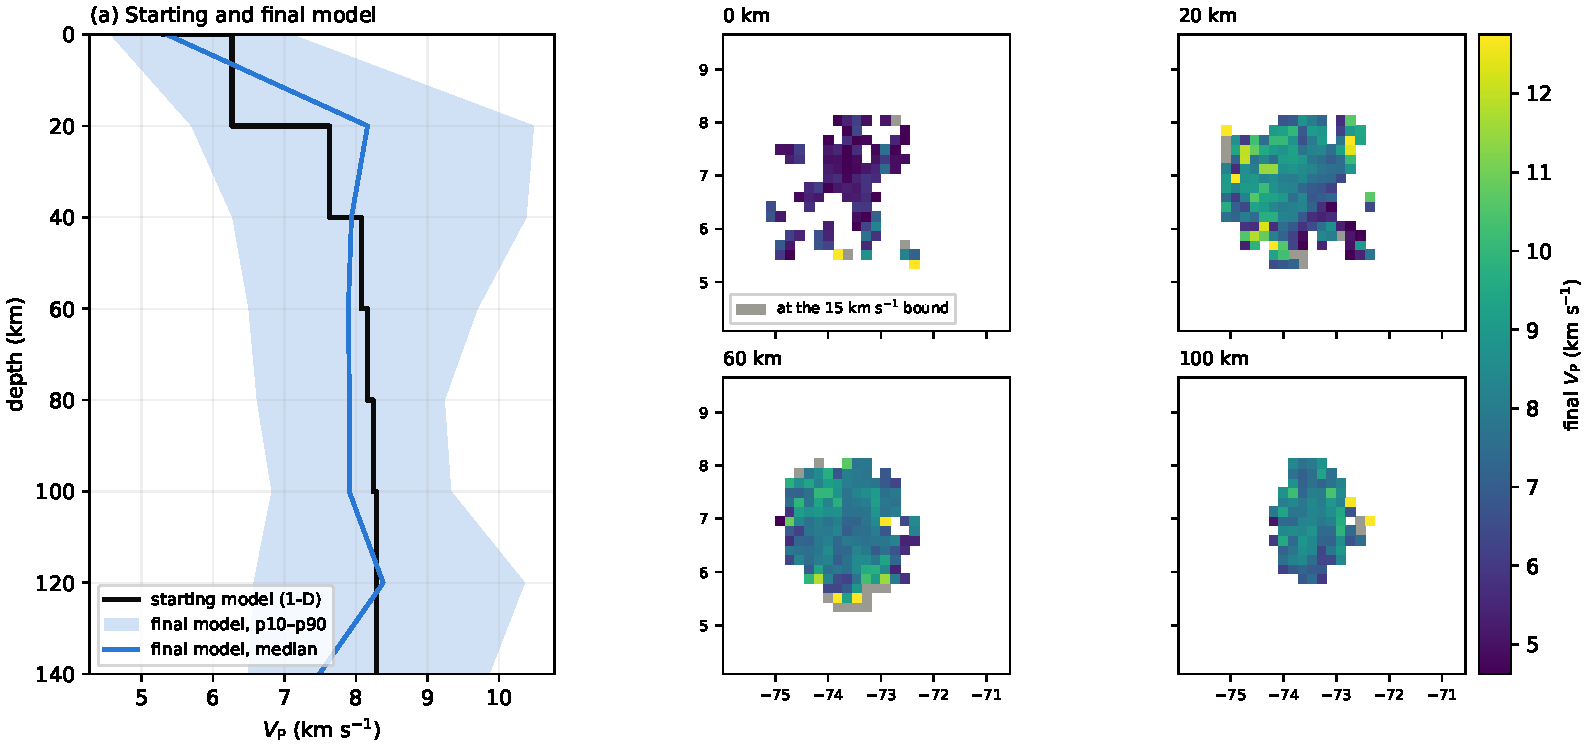
\includegraphics[width=1.0\linewidth]{modelos_vp.pdf}
  \caption{Starting and final P-wave velocity models. (a) The one-dimensional starting profile, with the median and the 10th--90th percentile range of the final model in each layer; the starting model is shown as a profile rather than as depth slices because it has no lateral structure. (b) Final model at four depths, restricted to active cells. Cells resting against the imposed upper bound on velocity (\SI{15}{\kilo\metre\per\second}) are shown in grey and excluded from the colour scale; they are a limit of the algorithm rather than a measurement, and are the velocity counterpart of the $Q$ ceiling of Section~\ref{sec:techo}.}
  \label{fig:modelos}
\end{figure}

\subsection{Regularisation and the adopted model}

The sweep reduces component inflation at limited cost in the linear fit:
$\lambda_{\tau}$ can be raised from \qStationDampPrevio{} to
\qStationDamp{} with normalised RMS reduction falling only from
\explMascaraRayos\,\% to \explAdoptada\,\%, while the trade-off ratios
fall from \razonEstrMascaraRayos{} to \razonEstrAdoptada{} and from
\razonEstMascaraRayos{} to \razonEstAdoptada. Further damping reduces the normalised RMS reduction as well as
component amplitudes; we retain
$\lambda_{\tau}=\qStationDamp$ as the adopted compromise (Fig.~\ref{fig:curvaL}).
The component correlation remains \corrComponentesAdoptada{}, compared
with \corrComponentesMascaraRayos{} at the original damping.
The paired conditional bootstrap change in $E_{\rm RMS}$ is
\auditDampingChange{} percentage points (95\,\% interval
\auditDampingChangeCI); the reduction is small but consistent across
event resamples of these fixed predictions.
Anticorrelation is reduced, but the partition is still strongly coupled.
Unity-scale ratios therefore do not justify calling the result well
conditioned or uniquely resolved. Figure~\ref{fig:estaciones} maps the
actual station terms. Damping can suppress genuine receiver response
as well as compensating terms; these data provide no independent
calibration that separates the two. The synthetic tests establish reduced
spurious leakage only for their declared structure-only inputs.

\begin{figure}[t]
  \centering
  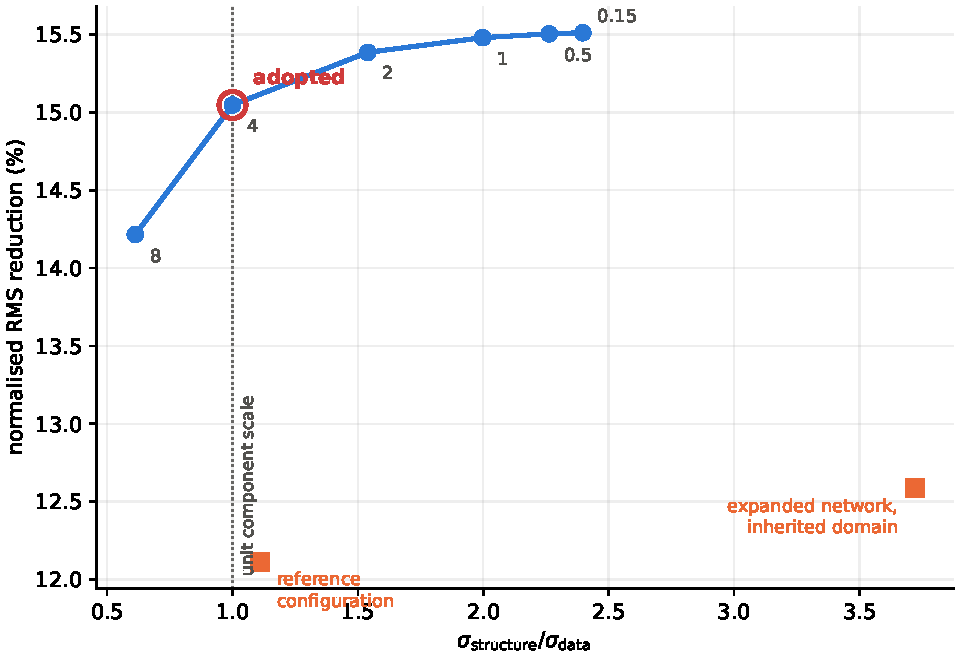
\includegraphics[width=0.70\linewidth]{curva_l.pdf}
  \caption{Trade-off between component inflation and linear fit. The abscissa is
  the standard deviation of the structural component of
  Equation~\ref{eq:descomp} normalised by that of the data; the ordinate
  is normalised RMS reduction relative to the data. Points are labelled by
  $\lambda_{\tau}$. The expanded network on the inherited domain lies far
  to the right, with components several times larger than the data and
  little normalised RMS reduction. The sweep traverses the curve leftwards; the
  compromise at $\lambda_{\tau}=\qStationDamp$ is adopted. Ratios
  near unity do not establish independence of the components.}
  \label{fig:curvaL}
\end{figure}

\begin{figure}[t]
 \centering
 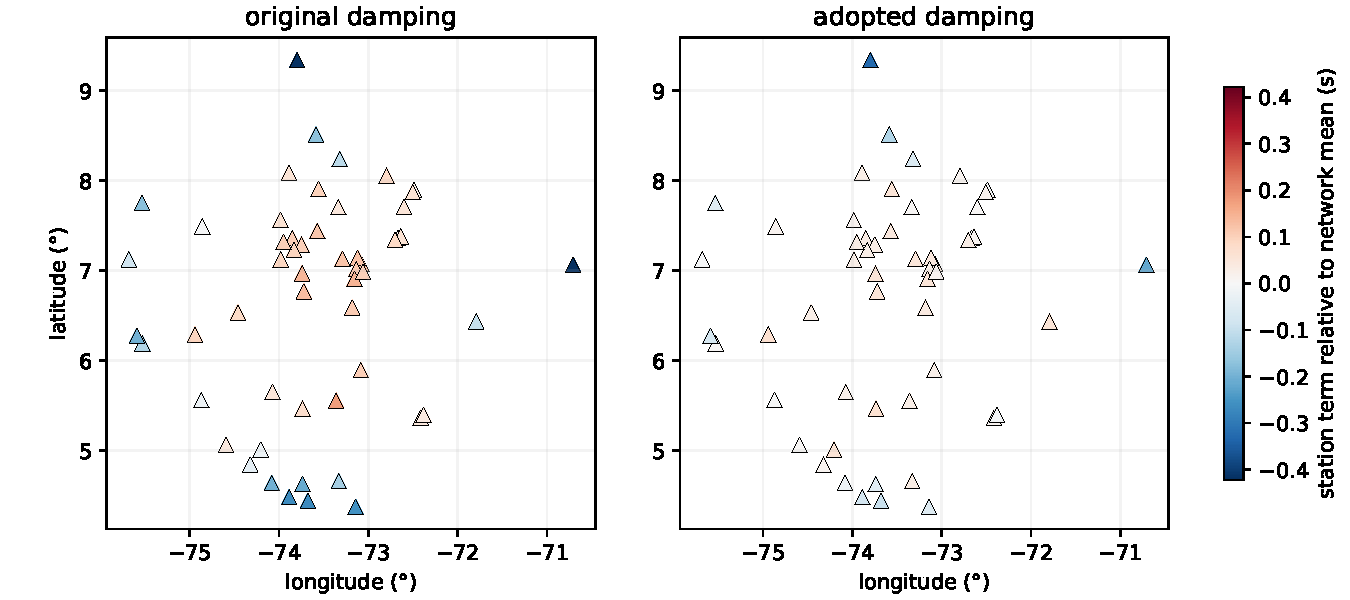
\includegraphics[width=1.0\linewidth]{terminos_estacion.pdf}
 \caption{Station terms on the ray-consistent domain at original and
 adopted damping, expressed relative to the network mean on a common
 colour scale. Only station differences enter the observations. The
 reduced amplitudes may include suppression of genuine receiver response;
 no independent site calibration is available to separate that effect
 from compensation for path structure.}
 \label{fig:estaciones}
\end{figure}

\subsection{Resolution}

Checkerboard recovery is summarised in Table~\ref{tab:damero}. The
velocity branch recovers the imposed pattern almost completely at low
noise ($r=\damVpBajoD$ at \SI{160}{\kilo\metre}) but degrades sharply at
the observed residual level ($r=\damVpObsD$), with amplitude ratios
exceeding unity, the expected behaviour when noise dominates. The
attenuation branch is markedly less noise-sensitive, falling only from
$r=\damQBajoD$ to $r=\damQObsD$ at \SI{160}{\kilo\metre}, and recovers the tested patterns at wavelengths of \SI{80}{\kilo\metre}
and longer on this fixed geometry. The \SI{80}{\kilo\metre} pattern
has four grid spacings per wavelength. Its recovery is a scale-dependent
synthetic result, not a claim that arbitrary structures at that scale
are identifiable or that clipped-model amplitudes are validated.

Because the synthetic data contain no station terms, any recovered
$\tau$ is spurious. Under the adopted regularisation these have standard
deviations of \damTermQObsD--\damTermQObsA~s, one order of magnitude below
the data. Repeating the test with the original
$\lambda_{\tau}=\qStationDampPrevio$ raises them to
\damViejoTermQObsD--\damViejoTermQObsA~s while simultaneously lowering
structural recovery at every wavelength (for example $r=\damViejoQObsD$
versus $r=\damQObsD$ at \SI{160}{\kilo\metre}). The adopted regularisation
therefore improves both quantities, independently of the criterion by
which it was chosen.

\begin{table}[t]
  \centering
  \caption{Checkerboard recovery (correlation, and amplitude ratio in
  parentheses) for imposed perturbations of \damPerturbVp\,\% in slowness
  and \damPerturbQ\,\% in $Q^{-1}$. The low-noise and residual-noise columns describe two stated noise
  scenarios; they are not guaranteed upper and lower bounds on actual resolution.}
  \label{tab:damero}
  \begin{tabular}{lcccc}
    \toprule
    & \multicolumn{2}{c}{$V_\mathrm{P}$}
    & \multicolumn{2}{c}{$Q$} \\
    \cmidrule(lr){2-3}\cmidrule(lr){4-5}
    $\lambda$ (km) & low noise & observed & low noise & observed \\
    \midrule
    40  & \damVpBajoA\ (\damAmpVpBajoA) & \damVpObsA\ (\damAmpVpObsA)
        & \damQBajoA\ (\damAmpQBajoA)   & \damQObsA\ (\damAmpQObsA) \\
    80  & \damVpBajoB\ (\damAmpVpBajoB) & \damVpObsB\ (\damAmpVpObsB)
        & \damQBajoB\ (\damAmpQBajoB)   & \damQObsB\ (\damAmpQObsB) \\
    120 & \damVpBajoC\ (\damAmpVpBajoC) & \damVpObsC\ (\damAmpVpObsC)
        & \damQBajoC\ (\damAmpQBajoC)   & \damQObsC\ (\damAmpQObsC) \\
    160 & \damVpBajoD\ (\damAmpVpBajoD) & \damVpObsD\ (\damAmpVpObsD)
        & \damQBajoD\ (\damAmpQBajoD)   & \damQObsD\ (\damAmpQObsD) \\
    \bottomrule
  \end{tabular}
\end{table}

\subsection{What the data determine about \texorpdfstring{$Q$}{Q}}
\label{sec:techo}

The archived RMS difference \cambioRmsTecho~s is expected from the
implementation and is not an independent ceiling test. Forward evaluation
of the saved clipped models instead yields \rmsQRecortado~s at
$Q_{\max}=\qTecho$ and \rmsQRecortadoAlto~s at
$Q_{\max}=\qTechoPrueba$, compared with \rmsFinalAdoptada~s for the
unconstrained linear prediction. The reported linear fit therefore cannot
be assigned to either bounded map.
Both clipped-model residual RMS values exceed the data RMS
\auditAdoptedDataRms~s: their $E_{\rm RMS}$ values are
\auditClippedLowE\,\% and \auditClippedHighE\,\%, respectively. Thus
the displayed maps, combined with the archived station terms, fit worse
than predicting zero differential attenuation. Velocity and station terms
are held fixed in both forward evaluations; re-estimating the station
terms after clipping could reduce these residuals. The two RMS values
compare different clips of the same unconstrained solution and are not
evidence favouring either ceiling.

At the original ceiling, \fracEnTecho\,\% of active nodes are clipped;
\fracVuelveATopar\,\% of those nodes reach the higher ceiling when it is
changed. The remaining \celdasLibresTecho{} nodes
(\fracCeldasLibres\,\%) have median $Q=\qLibreMediana$ and 10th--90th
percentiles \qLibreDiez--\qLibreNoventa. Their median changes by
\cambioQLibre\,\% because the same unconstrained solution is clipped
differently, not because a constrained inversion independently recovered
them. Being below the ceiling is necessary for considering a value, but
does not establish that it is constrained by the data. The maps are
therefore provisional descriptions of the clipped output.
At the other bound, \auditLowerBoundNodes{} active nodes
(\auditLowerBoundPercent\,\%) reach $Q=20$, both with the original and
the higher ceiling.

\begin{figure}[t]
  \centering
  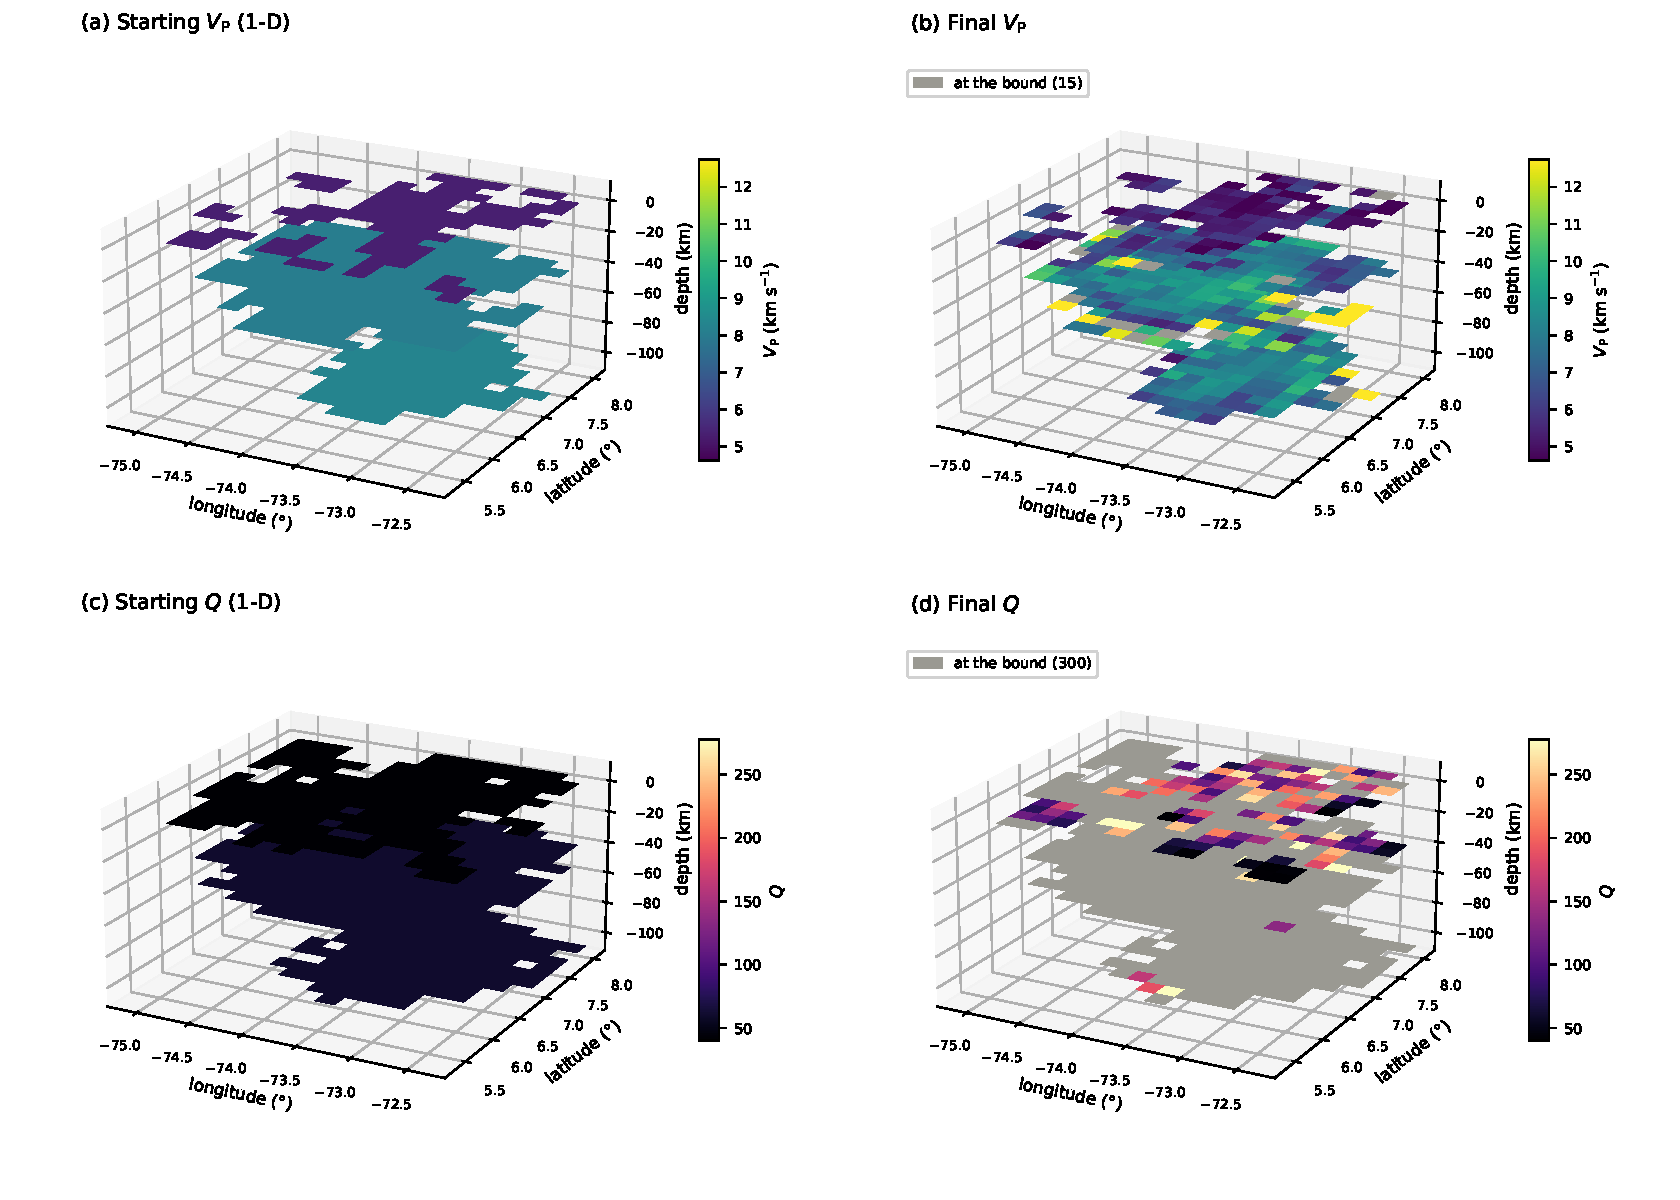
\includegraphics[width=1.0\linewidth]{volumenes_3d.pdf}
  \caption{Starting and final models in isometric view, shown as horizontal planes at 0, 40 and \SI{100}{\kilo\metre} and restricted to active cells. (a) and (c) are the one-dimensional starting models: lateral variation within each layer is zero to numerical precision for $V_\mathrm{P}$, and $Q$ takes only two values. Lateral departures from the starting models in (b) and (d) arise from the inversion, regularisation and subsequent clipping; they cannot all be attributed to data alone. In (b) and (d), cells resting against the imposed bounds on velocity and on $Q$ are shown in grey and excluded from the colour scale; their extent in (d) is the visual counterpart of the ceiling test of Section~\ref{sec:techo}.}
  \label{fig:volumenes}
\end{figure}

Below-ceiling nodes are not uniformly distributed (Fig.~\ref{fig:modelosq}). The proportion at the ceiling
is \fracTechoZSup\,\% at the surface and \fracTechoZCien\,\% at
\SI{100}{\kilo\metre}, so below-ceiling values are concentrated in the upper
crust. The medians over below-ceiling nodes within each depth layer are \qLibreZSup{} at the surface,
\qLibreZVeinte{} at \SI{20}{\kilo\metre} and \qLibreZCuarenta{} at
\SI{40}{\kilo\metre}.

\begin{figure}[t]
 \centering
 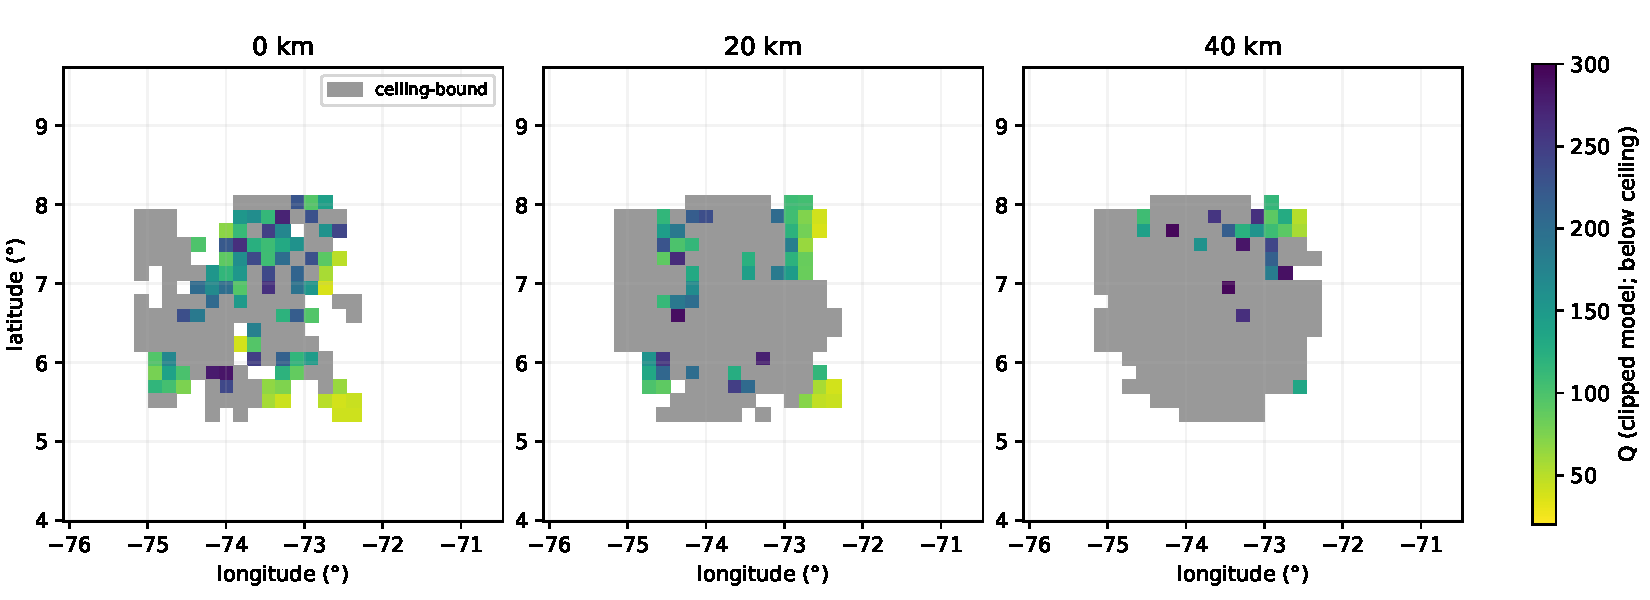
\includegraphics[width=1.0\linewidth]{modelos_q.pdf}
 \caption{Horizontal slices of the saved clipped attenuation model.
 Ceiling-bound active nodes are grey and inactive nodes are blank.
 The colour scale includes only below-ceiling values. These are provisional
 maps: their forward RMS differs from the archived unconstrained fit,
 and absence of clipping alone does not establish data support.}
 \label{fig:modelosq}
\end{figure}

\subsection{Benioff surface}

The surface is constrained by \losaControles{} hypocentres and spans
\losaProfMin--\losaProfMax~km depth over \losaNodos{} nodes, with a median
distance of \losaDistControl~km from any node to its nearest control.
Median local dip is \losaBuzamiento$^{\circ}$ (90th percentile
\losaBuzamientoNoventa$^{\circ}$); the single-plane trend of
\losaTendencia$^{\circ}$ is reported only for completeness, as it averages
across a curved surface. Compared with Slab2 over \slabNodos{} nodes, the
median signed difference is \slabDifMediana~km and the median absolute
difference \slabDifAbs~km, with a 90th percentile of \slabDifNoventa~km.

\begin{figure}[t]
  \centering
  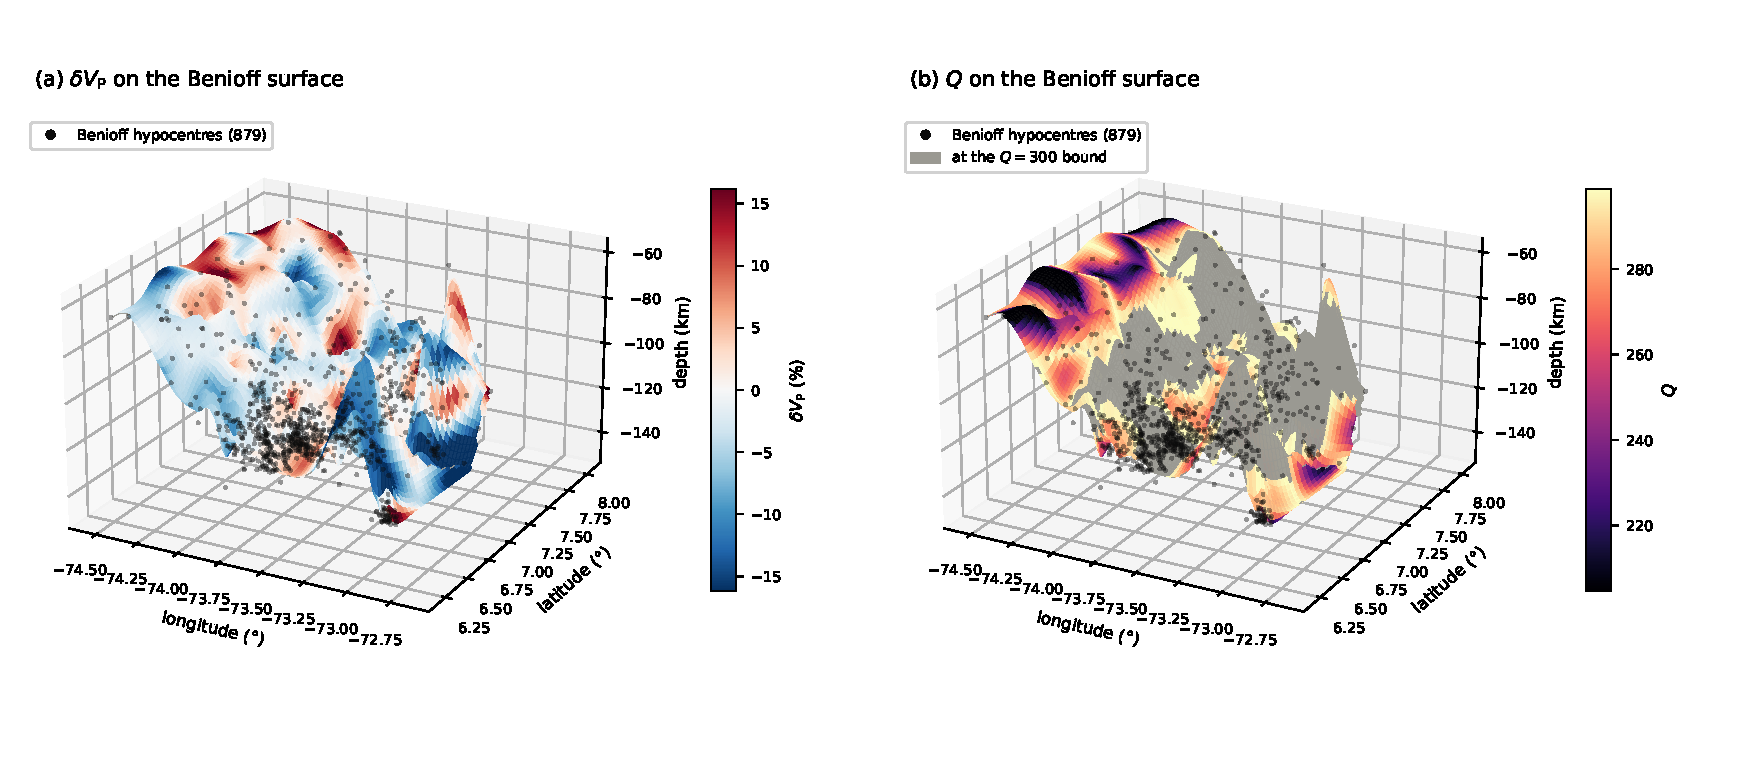
\includegraphics[width=1.0\linewidth]{losa_3d.pdf}
  \caption{Benioff surface in isometric view, reconstructed from \losaControles{} intermediate-depth hypocentres (black dots), with (a) the velocity anomaly and (b) $Q$ sampled on it as attributes. The geometry is defined by seismicity alone; neither field enters the surface fit. In (b) the nodes resting against the imposed $Q$ ceiling are shown in grey and excluded from the colour scale, following Section~\ref{sec:techo}; they cover a large part of the surface, so no quantitative attenuation interpretation is offered at intermediate depth. Trilinear attribute interpolation does not increase tomographic resolution.}
  \label{fig:losa}
\end{figure}

% =====================================================================
\section{Discussion}
% =====================================================================

\subsection{Illumination and parameterisation are distinct constraints}

In this dataset, the expanded campaign on an inherited domain increases
component inflation while producing little improvement in normalised
linear RMS reduction. Domain expansion and stronger station damping reduce
that inflation and improve structure-only synthetic recovery. The
remaining anticorrelation shows that the two contributions are still
coupled. Reporting their normalised amplitudes and covariance together is
more informative than either the initial-model RMS reduction or a
unity-scale amplitude criterion alone.

The result is a case study rather than a general argument against adding
receivers. Additional stations may improve identifiability when they add
independent path directions, when the domain already spans the illuminated
volume, or when site response is independently constrained. Dense networks
and different source distributions need not exhibit the same trade-off.
Here the spectral pairs share records, and the straight-ray approximation
and fixed hypocentres further restrict what can be inferred.

\subsection{Clipping must be distinguished from constrained inference}

Many nodes in the archived maps reach their numerical bounds, but the
recorded predictions belong to an unconstrained linear solution. The
ceiling comparison exposes a mismatch between the model displayed and the
model whose residual is reported. A fraction of ceiling-bound nodes is
still a useful diagnostic; however, unchanged pre-clipping RMS is not
evidence that the data permit arbitrarily high $Q$.
Neither the ceiling-bound nor the below-ceiling values can be labelled
measurements on the basis of this test. A bound-constrained inversion,
with predictions evaluated from its returned model and uncertainty or
sensitivity tests for the bounds, is required for that interpretation.

\subsection{Provisional attenuation structure of the basin}

Figure~\ref{fig:modelosq} displays the clipped attenuation output with
ceiling-bound nodes excluded from the colour scale. The medians over
below-ceiling nodes are \qLibreZSup{} at the surface,
\qLibreZVeinte{} at \SI{20}{\kilo\metre} and \qLibreZCuarenta{} at
\SI{40}{\kilo\metre}. Thus the quoted range
\qLibreZVeinte--\qLibreZCuarenta{} describes two layer medians,
not the range of individual values or the global median.
The global below-ceiling median is \qLibreMediana{}, with a much broader
10th--90th percentile interval \qLibreDiez--\qLibreNoventa.

Sedimentary basin fill and fluid-sensitive attenuation provide geological
hypotheses for these patterns \citep{Mavko2009,Biot1956,QuanHarris1997,
MojicaFranco1990,GomezTapias2019,Londono2022Attenuation,Castelblanco2025Attenuation}.
The present clipping audit, low spectral-fit quality and residual
station--structure coupling prevent validation of that interpretation.
We do not infer a fluid distribution or quantitative slab attenuation
from these maps \citep{EberhartPhillipsChadwick2002,JinEtAl2021}.

\subsection{Benioff geometry and velocity structure}

The reconstructed surface agrees with Slab2 to \slabDifAbs~km in median
absolute depth, providing a descriptive comparison with the external model
\citep{Hayes2018Slab2}. We have not evaluated a regional Slab2 uncertainty
field or propagated hypocentral errors, so this difference is not claimed
to lie within a quantified uncertainty interval.
Median local dip of \losaBuzamiento$^{\circ}$ is consistent with the
intermediate-depth segment beneath northeastern Colombia inferred from
regional seismicity \citep{Zarifi2007,SepulvedaJaimes2018,Syracuse2016}.
The velocity field sampled on the surface shows a localised low-velocity
anomaly within the Bucaramanga nest volume relative to its surroundings.
Interpretation at this scale is restricted by the velocity resolution of
Table~\ref{tab:damero}: at the observed noise level the velocity branch
recovers only $r\approx\damVpObsD$ even at \SI{160}{\kilo\metre}, so we
regard the displayed anomaly as tentative and do not interpret its
amplitude or sign as independently validated.

\subsection{Limitations}

The straight-ray operator and fixed hypocentres make this a linearised
audit rather than a fully non-linear tomography solution; finite-frequency
or eikonal modelling and relocation would change the kernels
\citep{Sethian1996,Zhao2005,Vavrycuk2012eikonal,Thurber1992}.
Velocity and attenuation maps are clipped after unconstrained optimisation,
and the fit reported for that optimisation is not their forward fit.
Checkerboards use the same operator as the inversion and therefore test
recovery within that discretisation, not robustness to ray bending,
model error or clipping. Independent Gaussian noise at the residual RMS
does not reproduce record sharing or correlated spectral errors, and
the two noise scenarios are not rigorous bounds on true resolution.
No uncertainty weighting, held-out prediction or independent station-response
calibration is available here. The fine Benioff surface grid likewise does
not justify fine-scale interpretation of interpolated tomographic fields.
These limitations prevent treating the clipped $Q$ values as quantitative
measurements, while leaving the archived linear trade-off comparison
and its synthetic leakage diagnostics informative.

% =====================================================================
\section{Conclusions}
% =====================================================================

\begin{enumerate}
 \item Increasing the receiver set from \estPrevia{} to \estAdoptada{}
stations and accepted spectral pairs from \qObsPrevia{} to
\qObsAdoptada{} accompanies a change in normalised RMS reduction only from
 \explPrevia\,\% to \explMascaraVieja\,\% while increasing cancellation
between the structural and station components. Starting velocity structure
and computational extent also differ, so this comparison cannot isolate
the effect of receiver expansion.
 \item The inherited domain omits \fracCeldasFuera\,\% of nodes hit in
 the sampled pairs, carrying \fracImpactosFuera\,\% of ray hits.
 The paired event-bootstrap gain is \auditDomainGain{} percentage points
 (95\,\% interval \auditDomainGainCI); at fixed inherited velocity the
 mask alone adds \auditMaskGainFixedVp{} points to the linear fit.
 Re-parameterisation and stronger station damping reduce component
 inflation and improve structure-only checkerboard recovery, but the
 adopted component correlation of \corrComponentesAdoptada{} shows
 that substantial coupling remains.
 \item The archived RMS is evaluated before clipping. Forward RMS of
 the clipped attenuation model is \rmsQRecortado~s, changing to
 \rmsQRecortadoAlto~s at the higher ceiling. The earlier equality of
 archived RMS therefore cannot demonstrate upper-bound non-identifiability.
 Below-ceiling values are provisional output, not validated measurements.
 \item A Benioff surface from \losaControles{} hypocentres differs from
 Slab2 by a median absolute \slabDifAbs~km. Its fine surface sampling does
 not improve the resolution of the interpolated tomographic attributes.
\end{enumerate}

The operational recommendations are to report the covariance of structural
and station contributions on the retained observations, to avoid using
archived RMS invariance as evidence of bound non-identifiability, and to
recompute forward predictions from the bounded model actually displayed.
These checks precede quantitative interpretation of attenuation values.

\section*{CRediT authorship contribution statement}
\textbf{R\'omulo Sandoval Fl\'orez:} Conceptualization, Methodology, Software, Validation, Formal analysis, Investigation, Resources, Data curation, Writing -- original draft, Writing -- review and editing, Visualization.
\textbf{Francisco H. Cabrera Zambrano:} Conceptualization, Methodology, Software, Validation, Formal analysis, Investigation, Resources, Data curation, Writing -- original draft, Writing -- review and editing, Visualization.
\textbf{Claudia Patricia Parra Medina:} Conceptualization, Methodology, Software, Validation, Formal analysis, Investigation, Resources, Data curation, Writing -- original draft, Writing -- review and editing, Visualization.

\section*{Funding}
This research did not receive any specific grant from funding agencies in the public, commercial, or not-for-profit sectors.

\section*{Declaration of competing interests}
The authors declare no competing interests.

\section*{Data Availability}
Earthquake catalogues, phase picks and waveforms are distributed by the Servicio Geol\'ogico Colombiano. Slab2 is distributed by the U.S. Geological Survey \citep{Hayes2018Slab2}. The processed campaign tables, saved models, numerical configuration, covariance diagnostics, conditional event-bootstrap outputs, and clipped-model forward-prediction audit are provided in Supplementary Material S1. The code and processed research data are archived as version 1.0.2 at \url{https://github.com/romusan/vp-q-tomography-audit/tree/v1.0.2} \citep{Sandoval2026VpQArchive}. The archive supports the audit from saved processed inputs; it does not include raw waveforms or constitute complete reproduction from waveform acquisition through spectral preprocessing. Regeneration of the separate checkerboard and Benioff experiments is outside the verified scope; their archived summaries are included.

\section*{Declaration of generative AI and AI-assisted technologies in the manuscript preparation process}
During the preparation of this work the authors used Codex to assist with language revision. After using this tool, the authors reviewed and edited the content as needed and take full responsibility for the content of the manuscript.

\section*{Acknowledgments}
The authors acknowledge Universidad ECCI (R.S.F.) and Universidad Militar Nueva Granada (C.P.P.M.) for their technical support.

\bibliographystyle{elsarticle-harv}
\bibliography{references}
\end{document}
